%% LaTeX2e class for student theses
%% sections/content.tex
%% 
%% Karlsruhe Institute of Technology
%% Institute for Program Structures and Data Organization
%% Chair for Software Design and Quality (SDQ)
%%
%% Dr.-Ing. Erik Burger
%% burger@kit.edu
%%
%% Version 1.3.2, 2017-08-01



\chapter{Design of a TDNN acoustic model}
To find a good design for a TDNN acoustics model, we had to make several design decisions. Most of the design decisions were justified by experiments, while some were taken from related work. This chapter summarizes the decisions made and the corresponding results. In some cases, we will also provide a comparison with a fully-connected network, which served as our experiment baseline. It should be noted that the experiments described in \cite{peddinti2015jhu} and \cite{peddinti2015reverberation} provided the main inspiration for this work, therefore we based some of our parameters on their result. 

\subsection{Neural Network Parameters}
This section focuses on parameters that are related to the neural network design. 
\subsubsection{Input Context and Features}
The input context of all our TDNN models is ${-13,9}$, which means the TDNN sees the current frame, thirteen frames in the past, and nine frames in the future. This parameter was taken from the smallest TDNN model described in \cite{peddinti2015reverberation}. 
\subsubsection{Count and Width of Layers}
The count of layers and width of each layer is one of the most important design parameters for neural networks. As in \cite{peddinti2015reverberation}, all our models use the same amount of channels for each TDNN unit. Only the count of observed time frames changes with each layer. \\ \\
\begin{minipage}{\linewidth}
	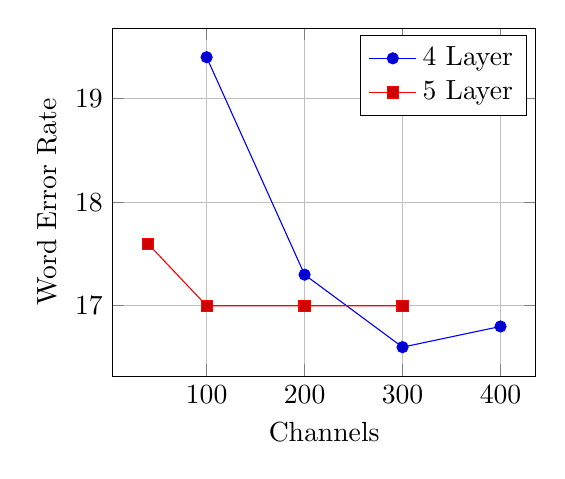
\begin{tikzpicture}
	\begin{axis}[ylabel=Word Error Rate, xlabel=Channels, height=6cm, 
	xticklabel style={name=T\ticknum},grid=major]
	\addplot coordinates {
		(100,19.4) %994
		(200,17.3) %999
		(300,16.6) %1009
		(400,16.8) %1010
	};
	\addlegendentry{4 Layer};
	\addplot coordinates {
		(40,17.6) %1040
		(100,17.0) %i3
		(200,17.0) %1039
		(300,17.0) %1036
	};
	\addlegendentry{5 Layer};
	\end{axis}
	\end{tikzpicture}
	\captionof{figure}{Word Error Rate for different choices of layer and channel count}
	\label{fig:tdnn_layer_design}
\end{minipage}
Figure \ref{fig:tdnn_layer_design} shows the word error rate for different configurations. The word error rate was estimated by using the same decoding parameters $l_p$ and $l_z$ for each architecture and the priors were estimated from the training data. Table \ref{tbl:tdnn_layer_design} gives the kernel size and stride over time for each layer in each architecture. \\ \\
\begin{minipage}{\linewidth}
	\centering 
	\begin{tabular} {|l | c | c | c | c | c | c | c | c | c | c | c | c |}
	\hline
	Model & \multicolumn{4}{c|}{4 Layer} & \multicolumn{5}{c|}{5 Layer} \\
	\hline
	Layer & 1 & 2 & 3 & 4 & 1 & 2 & 3 & 4 & 5 \\
	\hline
	Kernel Size & 5 & 2 & 2 & 2 & 5 & 5 & 3 & 2 & 2 \\
	\hline
	Stride & 3 & 2 & 2 & 2 & 2 & 1 & 1 & 1 & 1 \\
	\hline
	\end{tabular}
	\captionof{figure}{Splice and stride parameters for the two different architectures}
	\label{tbl:tdnn_layer_design}
\end{minipage}
For this set of experiments, each TDNN layer was followed by a LP-pooling nonlinearity with P of two and group size ten, as well as a batch normalization layer. 
\subsubsection{Nonlinearity}
Following\cite{zhang2014improving}, we use a LP-pooling nonlinearity with a P of two and a group size if ten after each TDNN layer. Using the LP norm can be problematic, as the gradient can become infinity when all inputs in the pooling group are zero. The authors of \cite{peddinti2015reverberation} propose to use a normalization layer after each LP-pooling layer, which solves the problem. We propose an alternate approach, which is setting the gradient to zero if all inputs become zero. Furthermore, we also tested max pooling as a possible nonlinearity. All experiments were conducted on the 4-Layer architecture described before. Figure \ref{fig:tdnn_nonlinearity} shows the results. 
\begin{minipage}{\linewidth}
	\begin{tikzpicture}
		\begin{axis}[
			   ybar,
			enlargelimits=0.15,
			legend style={at={(0.5,-0.2)},
				anchor=north,legend columns=-1},
			ylabel={\#participants},
			symbolic x coords={LP Batch Norm,MaxPool,LP Gradient Modification}
			%symbolic x coords={LP Batch Norm,MaxPool,LP Gradient Modificatoin},
			xtick=data,
			nodes near coords
		]
		
		% TODO: Fix this plot...
		\addplot coordinates {(LP Batch Norm,16.6) (MaxPool,15.8) 
			(LP Gradient Modification,15.5)};
	%	\addplot coordinates {1,16.6) (2,15.8) (3, 15.5)};
		%\addplot coordinates {(1,15.8)};
		%\addplot coordinates {(1,15.5)};
		
		%\legend{LP + Batch Norm, MaxPool, LP + Gradient Modification}
		\end{axis}
	\end{tikzpicture}
	\captionof{figure}{Word Error Rate for different choices of nonlinearities}
	\label{fig:tdnn_nonlinearity}
\end{minipage}
In our case, the usage of LP tuning with a modified gradient outperformed the other nonlinearities.  
\subsection{Training Parameters}

\subsection{Decoding Parameters}



\label{ch:approach}
This chapter describes our approach for acoustic modelling using TDNNs on a high level. 
We will also give a brief overview over unknown hyperparemters and design decisions,
as well as a coarse overview over the structure of our implementation. 

\chapter{Experiment Setup}
\label{ch:experiment_setup}
This chapter should describe the detailed preleminaries and hyperparemters of our training and evaluation setup:
\begin{itemize}
    \item which data, and which preprocessing was used
    \item how was the data reverbed
    \item which learning rate schedulers, optimizers, loss functions were used
    \item which mechanisms were used to make the training faster and scalable
\end{itemize}